\chapter{Cơ sở lý thuyết}
% \section{Cơ sở lý thuyết}

\section{Tổng quan bài toán về thị giác máy tính}
Thị giác máy tính (Computer Vision) là một lĩnh vực quan trọng của trí tuệ nhân tạo (AI), tập trung vào việc giúp máy tính hiểu, phân tích và diễn giải thông tin từ hình ảnh hoặc video. Mục tiêu của thị giác máy tính là mô phỏng khả năng quan sát và nhận thức của con người để trích xuất thông tin hữu ích phục vụ cho các ứng dụng như giám sát tự động, lái xe tự hành, y học chẩn đoán hình ảnh, hay tương tác người–máy.

Trong lĩnh vực này, có một số bài toán cơ bản và quan trọng như sau:

\textbf{Phân loại ảnh (Image Classification):} \\
Đây là bài toán gán một hoặc nhiều nhãn cho một bức ảnh dựa trên nội dung của nó. Mô hình được huấn luyện để nhận diện các đặc trưng phân biệt giữa các lớp ảnh. Các kiến trúc mạng nơ-ron tích chập (CNN) nổi bật như VGG, ResNet, DenseNet và EfficientNet đã đạt được những kết quả vượt trội trong bài toán này.

\textbf{Nhận diện đối tượng (Object Detection):} \\
Bài toán này không chỉ yêu cầu xác định loại đối tượng trong ảnh mà còn phải dự đoán vị trí của chúng thông qua các hộp giới hạn (bounding boxes). Các mô hình hiện đại như YOLO (You Only Look Once), SSD (Single Shot MultiBox Detector), và Faster R-CNN đã thể hiện hiệu quả cao cả về độ chính xác và tốc độ.

\textbf{Phân đoạn ảnh (Image Segmentation):} \\
Phân đoạn ảnh là quá trình chia ảnh thành các vùng có ý nghĩa, trong đó mỗi pixel được gán nhãn tương ứng với một đối tượng hoặc vùng cụ thể. Bài toán này cho phép mô hình hiểu cấu trúc chi tiết hơn trong ảnh so với nhận diện đối tượng. Một số mô hình tiêu biểu là U-Net, DeepLab và Mask R-CNN.

\textbf{Các bài toán nâng cao khác:} \\
Ngoài ba hướng trên, thị giác máy tính còn bao gồm nhiều bài toán khác như tái tạo ảnh 3D, ước lượng độ sâu, theo dõi đối tượng (object tracking), tăng cường ảnh (image enhancement) và sinh ảnh mới từ mô tả (text-to-image generation). Các bài toán này thường yêu cầu sự kết hợp giữa các mô hình học sâu và các kỹ thuật biểu diễn đặc trưng (feature representation) trong không gian tiềm ẩn (latent space).


\section{Mạng nơ-ron nhân tạo}
Mạng thần kinh nhân tạo (Artificial Neural Networks - ANN) là một mô hình tính toán lấy cảm hứng từ cách hoạt động của hệ thần kinh sinh học, đặc biệt là cấu trúc và chức năng của não bộ con người. ANN bao gồm các đơn vị tính toán gọi là nơ-ron nhân tạo, được kết nối với nhau theo nhiều tầng để xử lý thông tin và học từ dữ liệu.
\begin{figure}[H]
    \centering
    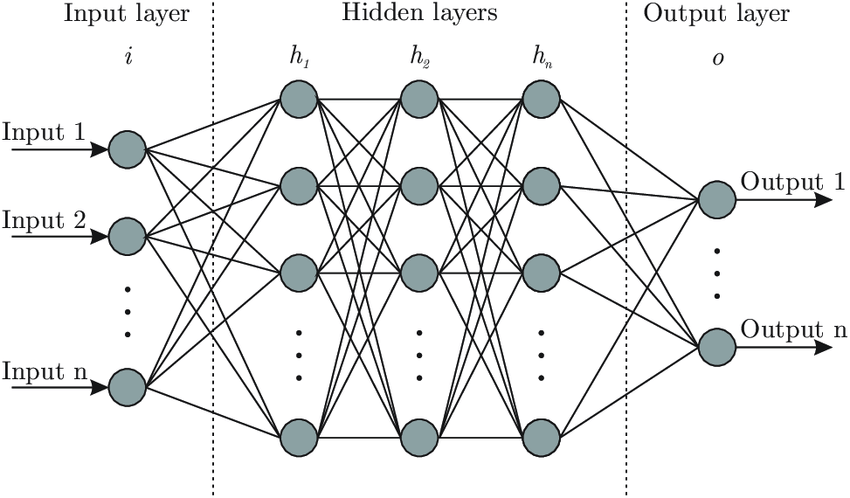
\includegraphics[width=0.5 \linewidth]{images/ANN.png}
    \caption{Kiến trúc ANN}
    \label{fig:ANN}
\end{figure}
Một ANN thông thường bao gồm các thành phần chính sau : 
\begin{itemize}
    \item \textbf{Tầng đầu vào : }Nhận dữ liệu đầu vào, có thể là hình ảnh, văn bản, âm thanh hoặc các dạng dữ liệu khác.
    \item \textbf{Tầng ẩn : }Bao gồm nhiều nơ-ron xử lý dữ liệu, áp dụng các phép toán và hàm kích hoạt để trích xuất đặc trưng từ dữ liệu.
    \item \textbf{Tầng đầu ra : }Tạo ra kết quả cuối cùng, có thể là nhãn phân loại, giá trị dự đoán, hoặc các thông tin khác tùy vào bài toán.
\end{itemize}
Nguyên lý hoạt động : 
Mỗi kết nối giữa các nơ-ron có một trọng số (weight) xác định mức độ ảnh hưởng của tín hiệu truyền qua. Khi dữ liệu đầu vào đi qua mạng, nó được tính toán qua các trọng số, cộng thêm một số bù (bias), và đi qua một hàm kích hoạt (activation function) để tạo ra đầu ra phi tuyến tính. Quá trình học của mạng thần kinh là tối ưu hóa các trọng số này thông qua các thuật toán như Lan truyền ngược (backpropagation) và Tối ưu hóa bằng lan truyền gradient (gradient descent).
\section{Mạng nơ-ron tích chập}
Mạng nơ-ron tích chập là một loại mạng nơ-ron nhân tạo chuyên xử lý dữ liệu dạng lưới, đặc biệt hiệu quả với ảnh và video. CNN mô phỏng cách hoạt động của vỏ não thị giác trong não người, giúp máy tính nhận diện và phân loại hình ảnh.

Khi xử lý ảnh màu RGB, CNN sử dụng các lớp tích chập để trích xuất đặc trưng. Ảnh đầu vào có ba kênh màu đỏ, lục, lam, được biểu diễn dưới dạng một tensor 3 chiều chiều cao, chiều rộng, số kênh. Mỗi bộ lọc trong lớp tích chập sẽ trượt qua ảnh, tính toán tích chập với từng kênh màu, sau đó tổng hợp kết quả để tạo ra một bản đồ đặc trưng.

Các lớp tích chập liên tiếp giúp mạng phát hiện các đặc trưng quan trọng như cạnh, góc, kết cấu và hình dạng. Tiếp theo, các lớp pooling giúp giảm kích thước dữ liệu, tăng hiệu quả tính toán. Cuối cùng, các lớp kết nối đầy đủ fully connected xử lý thông tin để thực hiện phân loại hoặc nhận diện đối tượng. Nhờ cơ chế này, CNN trở thành mô hình mạnh mẽ trong các ứng dụng như nhận diện khuôn mặt, phát hiện vật thể và phân loại hình ảnh.
\subsection{Ảnh màu RGB}
Ảnh màu RGB là một loại hình ảnh kỹ thuật số được biểu diễn bằng ba kênh màu cơ bản: Đỏ (Red - R), Xanh lá (Green - G) và Xanh dương (Blue - B). Hệ màu này dựa trên mô hình tổng hợp màu cộng (Additive Color Model), trong đó ba màu cơ bản được kết hợp với nhau theo các cường độ khác nhau để tạo ra nhiều màu sắc khác nhau.

Mỗi điểm ảnh (pixel) trong ảnh RGB được biểu diễn bằng một bộ ba giá trị tương ứng với cường độ sáng của từng kênh màu, thường có giá trị trong khoảng từ 0 đến 255 đối với ảnh 8-bit. Khi cả ba kênh đều đạt giá trị tối đa (255, 255, 255), điểm ảnh sẽ hiển thị màu trắng; khi cả ba kênh đều bằng 0 (0, 0, 0), điểm ảnh sẽ có màu đen. Sự thay đổi cường độ giữa ba kênh này cho phép tái tạo hàng triệu màu sắc khác nhau, tạo nên hình ảnh đa dạng và sinh động.

Trong xử lý ảnh, ảnh RGB thường được sử dụng như dữ liệu đầu vào cho các thuật toán nhận dạng, phân loại hoặc phát hiện đối tượng. Tuy nhiên, vì mỗi pixel chứa nhiều thông tin màu sắc, các kỹ thuật tiền xử lý như chuyển đổi ảnh về không gian màu khác (ví dụ: Grayscale, HSV) hoặc tách riêng từng kênh màu thường được áp dụng nhằm giảm độ phức tạp tính toán và tăng hiệu quả cho bài toán cụ thể.
\begin{figure}[H]
    \centering
    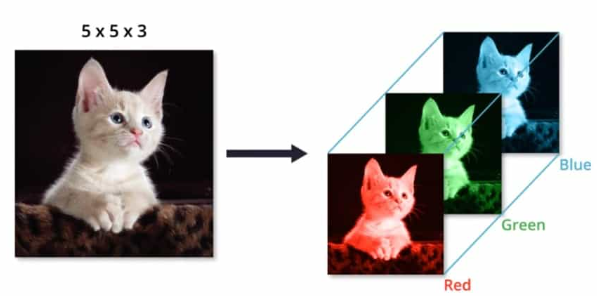
\includegraphics[width=0.4 \linewidth]{images/RGB.png}
    \caption{Ảnh màu RGB}
    \label{fig:RGB}
\end{figure}
\subsection{Lớp tích chập}
Lớp tích chập là thành phần cốt lõi của mạng nơ-ron tích chập, một mô hình chuyên dụng trong xử lý ảnh và thị giác máy tính. Lớp này có nhiệm vụ trích xuất đặc trưng từ ảnh bằng cách áp dụng các bộ lọc (kernels/filters) để phát hiện các mẫu như cạnh, góc, hình dạng hoặc kết cấu.

Cụ thể, mỗi bộ lọc trong lớp tích chập sẽ trượt trên toàn bộ ảnh đầu vào, thực hiện phép nhân điểm từng phần tử và tổng hợp lại thành một giá trị duy nhất, tạo ra một bản đồ đặc trưng cho mỗi bộ lọc. Các bộ lọc này ban đầu có trọng số ngẫu nhiên và được tối ưu hóa trong quá trình huấn luyện thông qua thuật toán lan truyền ngược nhằm học ra những mẫu quan trọng nhất cho bài toán.

Nhờ khả năng học các đặc trưng không cần thiết kế thủ công, lớp tích chập giúp mạng nơ-ron tự động phát hiện các yếu tố từ đơn giản (như đường biên) đến phức tạp (như cấu trúc đối tượng) qua nhiều tầng tích chập liên tiếp. Đây chính là lý do mạng nơ-ron tích chập đạt hiệu quả vượt trội trong các bài toán nhận dạng hình ảnh, phân loại ảnh, phát hiện đối tượng và nhiều ứng dụng thị giác máy tính khác.



\begin{figure}[H]
    \centering
    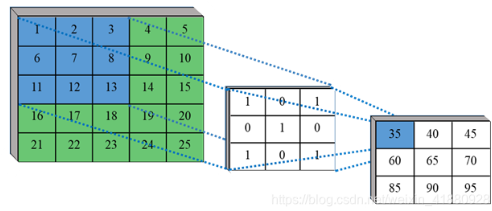
\includegraphics[width=0.5 \linewidth]{images/Kernel.png}
    \caption{Lớp tích chập trong trích xuất đặc trưng}
    \label{fig:convo}
\end{figure}

Cách hoạt động của lớp tích chập:

\begin{enumerate}
\item Duyệt một bộ lọc nhỏ qua từng vùng trên ảnh đầu vào
\item Nhân từng giá trị của bộ lọc với giá trị tương ứng của ảnh, sau đó cộng lại để tạo ra giá trị mới
\item Kết quả là một ma trận đầu ra (feature map) chứa các đặc trưng quan trọng của ảnh
\end{enumerate}

Công thức tích chập giữa ảnh đầu vào I và bộ lọc K : \\
\[
O(x, y) = \sum_{i}\sum_{j} I(x+i, y+j) \cdot K(i, j)
\]
Trong đó : 
\begin{itemize}
    \item $O(x, y)$ là giá trị tại tọa độ $(x,y)$ của ảnh
    \item $I(x+i, y+j)$ là giá trị điểm ảnh đầu vào
    \item $K(i,j)$ là giá trị của bộ lọc
\end{itemize}
\subsection{Tích chập chuyển vị}

Trong các mạng CNN, phép tích chập thường làm giảm kích thước không gian của đặc trưng. Ngược lại, tích chập chuyển vị giúp tăng kích thước đặc trưng, hữu ích trong các bài toán như phân đoạn ảnh hoặc siêu phân giải.

Về nguyên lý, tích chập chuyển vị chèn các giá trị zero giữa các pixel của đầu vào và thực hiện convolution với kernel, cho phép mở rộng không gian mà vẫn học được các trọng số thích nghi. Nếu đầu vào có kích thước $n$, kernel kích thước $k$, stride $s$ và padding $p$, kích thước đầu ra là:
\[
n_{out} = (n - 1) \times s - 2p + k
\]

\begin{figure}[H]
    \centering
    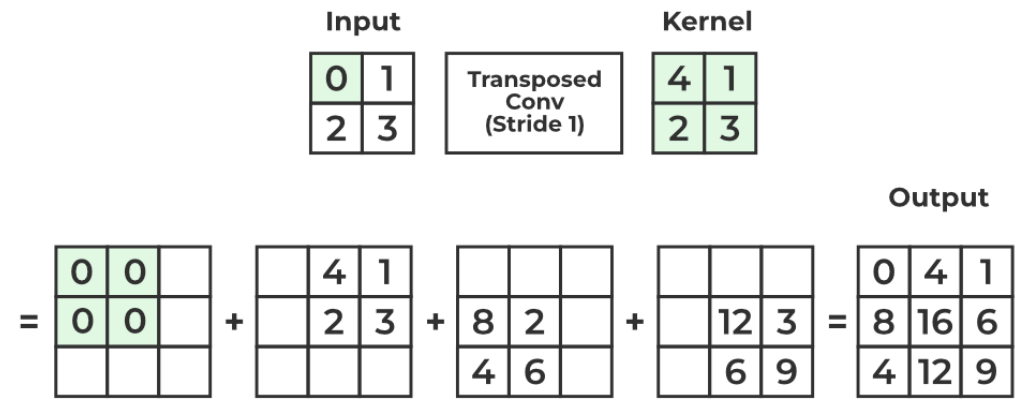
\includegraphics[width=0.6 \linewidth]{images/Kernel_transpose.png}
    \caption{Cách tính tích chập chuyển vị}
    \label{fig:convo_transpose}
\end{figure}
\subsection{Lớp pooling}
Lớp pooling là một thành phần quan trọng trong mạng nơ-ron tích chập, giúp giảm kích thước của dữ liệu đầu ra từ lớp tích chập, đồng thời giữ lại các đặc trưng quan trọng. Lớp này giúp tăng hiệu quả tính toán, giảm số lượng tham số và hạn chế tình trạng overfitting.

Có hai loại pooling phổ biến là max pooling và average pooling. Trong đó, max pooling chọn giá trị lớn nhất trong mỗi vùng nhỏ của ảnh đầu vào, giúp làm nổi bật các đặc trưng mạnh nhất như cạnh hoặc điểm nổi bật. Average pooling thì tính giá trị trung bình trong vùng đó, giúp làm mượt đặc trưng và giữ lại thông tin tổng quát.

Pooling còn có vai trò tạo ra sự bất biến đối với dịch chuyển nhỏ của đối tượng trong ảnh. Điều này có nghĩa là, nếu đối tượng trong ảnh bị dịch nhẹ sang trái, phải, lên hoặc xuống thì đặc trưng trích xuất sau lớp pooling vẫn không thay đổi nhiều. Nhờ đó, mô hình trở nên ổn định và chính xác hơn trong thực tế.

Thông thường, lớp pooling được đặt sau một hoặc nhiều lớp tích chập, và lặp lại nhiều lần trong toàn bộ kiến trúc của mạng để dần giảm kích thước không gian của ảnh đầu vào trong khi vẫn giữ được thông tin cần thiết cho việc phân loại hoặc nhận dạng.

\begin{figure}[H]
    \centering

    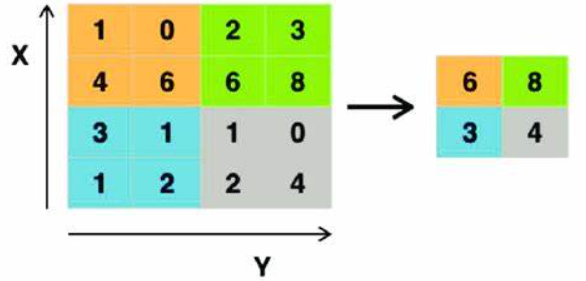
\includegraphics[width=0.5 \linewidth]{images/pooling.png}
    \caption{Lớp pooling trong mạng nơ-ron tích chập}
    \label{fig:pooling}
\end{figure}

Cách hoạt động của lớp pooling:

\begin{enumerate}
\item Chia ma trận đầu vào thành các vùng nhỏ không trùng lặp
\item Áp dụng phép toán (max pooling hoặc average pooling) lên từng vùng để lấy giá trị đại diện
\item Kết quả là một ma trận có kích thước nhỏ hơn nhưng vẫn giữ được các đặc trưng quan trọng
\end{enumerate}

Công thức của max pooling trên vùng kích thước \( k \times k \) được biểu diễn như sau:\\
\[
O(x, y) = \max_{i=0}^{k-1} \max_{j=0}^{k-1} I(x+i, y+j)
\]
Trong đó:
\begin{itemize}
    \item $O(x, y)$ là giá trị tại tọa độ $(x, y)$ của ma trận đầu ra.
    \item $I(x+i, y+j)$ là giá trị điểm ảnh đầu vào trong cửa sổ pooling.
\end{itemize}

\subsection{Hàm kích hoạt ReLU}

Hàm kích hoạt ReLU (Rectified Linear Unit) được sử dụng rộng rãi trong các mạng nơ-ron tích chập nhờ tính đơn giản và hiệu quả trong việc huấn luyện các mô hình sâu. ReLU được định nghĩa như sau:
\[
\mathrm{ReLU}(x) = \max(0, x)
\]

Trong mạng CNN, ReLU thường được áp dụng ngay sau mỗi lớp tích chập. Vai trò của nó là \textbf{giới thiệu tính phi tuyến (non-linearity)} vào mô hình, cho phép mạng học được các biểu diễn phức tạp hơn của dữ liệu đầu vào. Nếu chỉ sử dụng các phép tích chập tuyến tính mà không có hàm kích hoạt phi tuyến, toàn bộ mạng sẽ chỉ tương đương với một phép biến đổi tuyến tính duy nhất, khiến khả năng biểu diễn của mạng bị hạn chế.

\paragraph{Ý nghĩa của ReLU trong CNN}
\begin{itemize}
  \item \textbf{Tăng tốc huấn luyện:} ReLU giúp mạng hội tụ nhanh hơn so với các hàm kích hoạt truyền thống như sigmoid hay tanh, nhờ gradient không bị bão hòa trong vùng dương.
  \item \textbf{Giảm hiện tượng vanishing gradient:} Trong khi sigmoid/tanh làm gradient nhỏ dần khi lan truyền ngược qua nhiều lớp, ReLU giữ gradient = 1 với giá trị dương, giúp tín hiệu học được duy trì sâu trong mạng.
  \item \textbf{Tạo đặc trưng thưa (sparse feature map):} Với các giá trị âm bị triệt tiêu về 0, ReLU làm cho các feature map có nhiều phần tử bằng 0, giúp giảm tương quan giữa các đặc trưng và tăng tính khái quát hóa.
\end{itemize}

\paragraph{Hạn chế và giải pháp:}
Một nhược điểm phổ biến của ReLU trong CNN là hiện tượng \textbf{``ReLU chết'' (Dead ReLU)}, xảy ra khi một neuron luôn nhận giá trị âm nên đầu ra luôn bằng 0, không thể học được nữa. Để khắc phục, các biến thể như \textbf{Leaky ReLU}, \textbf{PReLU}, hoặc \textbf{ELU} thường được sử dụng.

\paragraph{Vị trí của ReLU trong kiến trúc CNN}
ReLU thường được đặt:
\begin{itemize}
  \item Sau mỗi lớp tích chập (Conv + ReLU)
  \item Sau mỗi lớp fully-connected (Linear + ReLU)
  \item Kết hợp với Batch Normalization để ổn định huấn luyện và tránh mất cân bằng giá trị đầu ra
\end{itemize}

\begin{figure}[H]
    \centering
    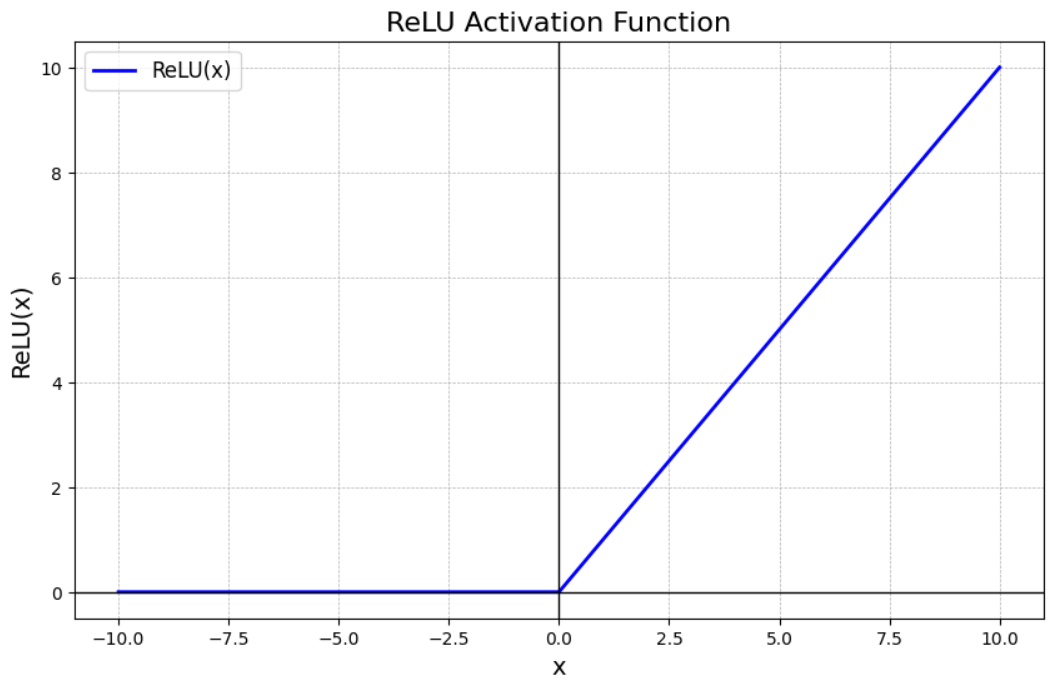
\includegraphics[width=0.6\textwidth]{images/ReLU.png}

    \caption{Hàm kích hoạt ReLU}
    \label{fig:relu_cnn}
\end{figure}

\section{Kiến trúc mô hình ResNet-50}

ResNet-50 là mạng nơ-ron tích chập sâu gồm 50 lớp, được xây dựng dựa trên các residual block nhằm giải quyết vấn đề suy giảm gradient khi huấn luyện mạng sâu. Kiến trúc ResNet-50 được chia thành các stage chính như sau:

\begin{itemize}
    \item \textbf{Stage 1 (Stem):} Gồm một lớp tích chập $7 \times 7$ với stride 2, theo sau là Batch Normalization, ReLU và Max Pooling $3 \times 3$. Stage này có nhiệm vụ trích xuất đặc trưng mức thấp từ ảnh đầu vào.
    
    \item \textbf{Stage 2 (Conv2\_x):} Bao gồm 3 residual bottleneck blocks. Mỗi block sử dụng cấu trúc $1 \times 1 \rightarrow 3 \times 3 \rightarrow 1 \times 1$, với số kênh đầu ra là 256.
    
    \item \textbf{Stage 3 (Conv3\_x):} Gồm 4 bottleneck blocks, tăng số kênh lên 512 và giảm kích thước không gian thông qua stride 2 ở block đầu tiên.
    
    \item \textbf{Stage 4 (Conv4\_x):} Bao gồm 6 bottleneck blocks, là stage sâu nhất của ResNet-50, với số kênh đầu ra là 1024.
    
    \item \textbf{Stage 5 (Conv5\_x):} Gồm 3 bottleneck blocks cuối cùng, mở rộng số kênh lên 2048 để trích xuất đặc trưng mức cao.
\end{itemize}

Cuối mạng là lớp Global Average Pooling và một lớp Fully Connected, thường được sử dụng cho bài toán phân loại. Trong các bài toán thị giác máy tính như Super Resolution, phần backbone ResNet-50 thường được sử dụng đến một stage nhất định để trích xuất đặc trưng \citep{he2016deep}.


\section{Lý thuyết về Entropy và ứng dụng trong mạng nơ-ron tích chập}

\subsection{Lý thuyết Entropy}

\subsubsection{Định nghĩa Entropy:}


Theo lý thuyết thông tin của Shannon \citep{shannon1948}, entropy là một đại lượng đo lường lượng thông tin hoặc độ bất định của một biến ngẫu nhiên. Đối với một biến ngẫu nhiên liên tục \(X\) trong không gian \(\mathbb{R}^{d}\) với hàm mật độ xác suất (pdf) \(f\), \textbf{entropy vi phân} (differential entropy) được định nghĩa là:

\begin{equation}
H(X) = \mathbb{E}\left[-\log f(X)\right]
\end{equation}


Công trình của Cover và Thomas \citep{cover2006} đã cung cấp nền tảng toán học vững chắc cho việc ứng dụng lý thuyết thông tin vào các lĩnh vực khác nhau, bao gồm cả học máy.

\subsubsection{Ý nghĩa của Entropy trong Mạng Neural:}

Trong bối cảnh của mạng neural, entropy của một tensor ẩn (hidden tensor) đại diện cho \textbf{mức độ đa dạng và phong phú của thông tin} mà tensor đó mang theo \citep{gabrie2018, meni2023}:

\begin{itemize}
    \item \textbf{Entropy cao}: Dữ liệu rất đa dạng và chi tiết, chứa đựng nhiều thông tin phong phú \citep{principe2000}. Biểu diễn này có nhiều trạng thái khả dĩ khác nhau.
    \item \textbf{Entropy thấp}: Dữ liệu trở nên tập trung hơn vào các đặc điểm chính, và do đó kém đa dạng hơn \citep{tishby1999}. Thông tin đã được nén lại hoặc lọc bớt, thường tập trung vào các đặc trưng quan trọng nhất cho tác vụ.
\end{itemize}

Việc theo dõi sự thay đổi của entropy khi dữ liệu truyền qua các lớp của mạng cho phép chúng ta hiểu được \textbf{cách mạng xử lý và chuyển hóa thông tin} \citep{erdogmus2003}.

\subsection{Sự Thay đổi Entropy trong lớp tích chập}

\subsubsection{Công thức tính toán:}

Một đóng góp quan trọng của bài báo \citep{meni2023} là biến đổi phép tích chập 2D thành một phép nhân ma trận-vector. Bằng cách "làm phẳng" (flatten) ảnh đầu vào \(X\) thành vector \(X_F\) và xây dựng một ma trận \(C_M\) đặc biệt từ bộ lọc tích chập \(C\), phép tích chập có thể được biểu diễn dưới dạng \(Z_F = C_M X_F\).

Sự thay đổi entropy khi áp dụng một bộ lọc tích chập \(C\) kích thước \(p \times q\) lên một đầu vào 2D \(X\) kích thước \(l \times w\) được tính bằng công thức sau \citep{meni2023}:

\begin{equation}
\Delta H_{\text{conv}} = (l - p + 1)(w - q + 1) \log(|c_{11}|)
\end{equation}

Trong đó \(c_{11}\) là \textbf{trọng số ở góc trên bên trái} của bộ lọc tích chập.

\subsubsection{Phân tích ý nghĩa và ảnh hưởng đến thông tin:}

Công thức (2) cho thấy sự thay đổi entropy \textbf{không phụ thuộc vào giá trị đầu vào} \(X\), mà chỉ phụ thuộc vào kích thước và một trọng số cụ thể của bộ lọc \citep{meni2023}. Điều này có ý nghĩa quan trọng:

\paragraph{Ảnh hưởng của \( \log(|c_{11}|) \)}:

Giá trị và dấu của \(\log(|c_{11}|)\) quyết định \textbf{hướng thay đổi thông tin cho mỗi điểm ảnh} trong bản đồ đặc trưng đầu ra \citep{meni2023}:

\begin{itemize}
    \item \textbf{Nếu \(|c_{11}| > 1\)}: Khi đó \(\log(|c_{11}|) > 0\). Bộ lọc có xu hướng \textbf{khuếch đại tín hiệu và nhiễu} từ đầu vào, làm tăng entropy và tính đa dạng của thông tin. Nó có "tiềm năng" tạo ra các biểu diễn phong phú hơn \citep{gabrie2018}.
    \item \textbf{Nếu \(|c_{11}| < 1\)}: Khi đó \(\log(|c_{11}|) < 0\). Bộ lọc có xu hướng \textbf{giảm cường độ tín hiệu}, làm dịu (smoothing) và nén thông tin, dẫn đến giảm entropy \citep{tishby1999}. Nó có "tiềm năng" lọc bỏ nhiễu và tập trung vào các đặc trưng nổi bật.
    \item \textbf{Nếu \(|c_{11}| = 1\)}: Khi đó \(\log(|c_{11}|) = 0\). Về mặt lý thuyết, thành phần này không làm thay đổi entropy.
\end{itemize}

\paragraph{Ảnh hưởng của hệ số \((l - p + 1)(w - q + 1)\):}

Hệ số này phản ánh \textbf{tổng số lần bộ lọc được áp dụng} (số "cửa sổ" trượt) để tạo ra toàn bộ bản đồ đặc trưng đầu ra. Nó \textbf{khuếch đại hiệu ứng} của \(c_{11}\) lên toàn bộ bản đồ đặc trưng \citep{meni2023}.

\subsubsection{Kết luận:}

Việc tính toán được \(\Delta H_{\text{conv}}\) một cách rõ ràng và hiệu quả cho phép chúng ta không chỉ theo dõi mà còn \textbf{chủ động hướng dẫn dòng thông tin} trong mạng \citep{meni2023}. Bằng cách thêm các hàm mất mát dựa trên \(\Delta H\) (ví dụ: khuyến khích bảo toàn thông tin ở các lớp đầu và nén thông tin ở các lớp cuối), chúng ta có thể "dạy" cho mạng học các kiểu lan truyền entropy lý tưởng, từ đó giúp mạng:


\section{Phương pháp Autoencoder}
\label{sec:ae_theory}

Mã hóa tự động (Autoencoder) là một mô hình học sâu deep learning được thiết kế để học biểu diễn nén của dữ liệu đầu vào mà không cần nhãn. Cấu trúc của một Autoencoder bao gồm hai phần chính: \textbf{bộ mã hóa (encoder)} và \textbf{bộ giải mã (decoder)}. 

\begin{figure}[H]
    \centering
    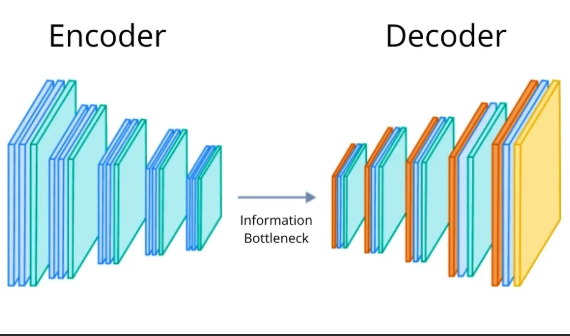
\includegraphics[width=0.6\textwidth]{images/autoencoder.png}
    \caption{Kiến trúc Autoencoder}
    \label{fig:autoencoder}

\end{figure}


\begin{itemize}
    \item \textbf{Bộ mã hóa (Encoder)}: có nhiệm vụ biến đổi dữ liệu đầu vào $x$ thành một biểu diễn có chiều thấp hơn, gọi là vector đặc trưng ẩn $z$. Quá trình này tương đương với việc trích chọn những đặc trưng quan trọng nhất của dữ liệu.
    \item \textbf{Bộ giải mã (Decoder)}: tái tạo lại dữ liệu đầu vào $\hat{x}$ từ biểu diễn ẩn $z$, sao cho $\hat{x}$ gần giống với $x$ ban đầu nhất có thể.
\end{itemize}



Mục tiêu huấn luyện của Autoencoder là tối thiểu hóa sai số giữa đầu vào và đầu ra tái tạo, thường được biểu diễn bởi hàm mất mát bình phương trung bình (Mean Squared Error):
\[
L(x, \hat{x}) = \| x - \hat{x} \|^2
\]

Trong các bài toán về thị giác máy tính, đặc biệt là xử lý ảnh, Autoencoder thường được triển khai dựa trên mạng nơ-ron tích chập. Khi đó, các lớp tích chập trong phần encoder giúp trích xuất đặc trưng không gian của ảnh, trong khi các lớp giải chập (deconvolution hoặc transpose convolution) trong phần decoder đảm nhiệm việc tái tạo ảnh từ các đặc trưng đã nén.


Nhờ khả năng học biểu diễn đặc trưng một cách không giám sát, Autoencoder đã trở thành nền tảng cho nhiều mô hình hiện đại trong thị giác máy tính, như siêu phân giải, khử nhiễu ảnh, và phát hiện bất thường. Khi được huấn luyện cùng các kiến trúc CNN sâu, Autoencoder giúp mô hình trích chọn được các đặc trưng ngữ nghĩa và không gian mạnh mẽ hơn, cải thiện đáng kể chất lượng ảnh đầu ra.

\section{Phương pháp GAN}
\label{sec:gan_theory}

Generative Adversarial Network (GAN) là một mô hình học sâu gồm hai thành phần chính: bộ sinh (Generator) và bộ phân biệt (Discriminator). Hai mô hình này được huấn luyện theo cơ chế đối kháng: Generator cố gắng tạo ra dữ liệu tổng hợp sao cho giống dữ liệu thật nhất có thể, trong khi Discriminator cố gắng phân biệt đâu là dữ liệu thật và đâu là dữ liệu do Generator sinh ra. Quá trình tối ưu ngược mục tiêu này tạo ra một vòng lặp cạnh tranh, giúp Generator dần học được phân phối của dữ liệu thật và sinh ra kết quả có chất lượng cao.
\begin{figure}[H]
    \centering
    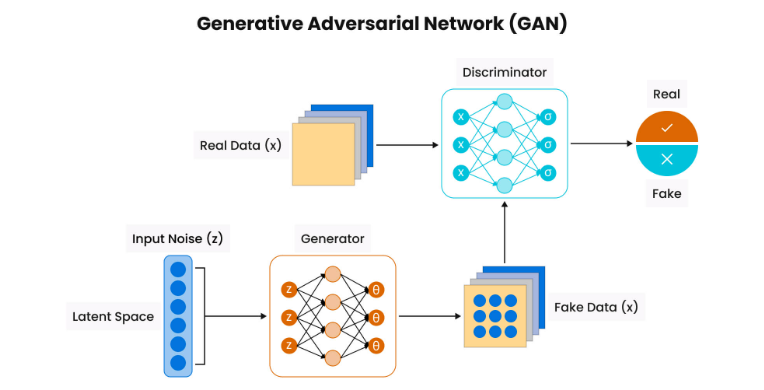
\includegraphics[width=1\textwidth]{images/GAN.png}
    \caption{Kiến trúc GAN}
    \label{fig:autoencoder}

\end{figure}
Trong bài toán khử nhiễu ảnh, GAN thường được sử dụng như một mô hình sinh học nhằm tái tạo ảnh sạch từ ảnh bị nhiễu. Thay vì chỉ tối ưu theo hàm mất mát truyền thống như MSE hoặc MAE, GAN bổ sung thêm thành phần mất mát đối kháng (adversarial loss) để khuyến khích ảnh tái tạo có tính chân thực cao hơn. Điều này giúp mô hình phục hồi được các cấu trúc chi tiết, biên cạnh và hoa văn phức tạp mà các phương pháp khử nhiễu truyền thống thường làm mờ.

Cụ thể, Generator nhận đầu vào là ảnh nhiễu và sinh ra ảnh sạch dự đoán. Discriminator đánh giá xem ảnh đầu ra có giống ảnh thật hay không. Thông qua quá trình huấn luyện, Generator không chỉ cố gắng giảm sai số điểm ảnh mà còn học cách sinh ảnh giống thật theo đặc trưng phân phối mà Discriminator học được từ dữ liệu sạch. Nhờ đó, các mô hình GAN được chứng minh là mang lại chất lượng thị giác tốt hơn so với các phương pháp dựa trên tối ưu điểm ảnh đơn thuần.

Về mặt tối ưu, hàm mất mát của GAN trong bài toán khử nhiễu ảnh thường được xây dựng
dưới dạng hàm tổng hợp, bao gồm thành phần mất mát tái tạo theo điểm ảnh và thành phần
mất mát đối kháng. Cụ thể, hàm mất mát đối kháng được định nghĩa như sau:
\begin{equation}
\mathcal{L}_{\text{adv}} =
\mathbb{E}_{x \sim p_{\text{clean}}(x)} [\log D(x)] +
\mathbb{E}_{y \sim p_{\text{noisy}}(y)} [\log (1 - D(G(y)))]
\end{equation}
trong đó $x$ là ảnh sạch, $y$ là ảnh bị nhiễu, $G(y)$ là ảnh sạch dự đoán do bộ sinh tạo ra,
và $D(\cdot)$ là xác suất mà bộ phân biệt gán cho đầu vào là ảnh thật.

Bên cạnh đó, để đảm bảo ảnh khôi phục giữ được độ chính xác theo điểm ảnh,
một hàm mất mát tái tạo $\mathcal{L}_{\text{rec}}$ (chẳng hạn như MSE hoặc MAE)
được sử dụng:
\begin{equation}
\mathcal{L}_{\text{rec}} =
\mathbb{E}_{x,y} [ \| G(y) - x \| ]
\end{equation}

Từ đó, hàm mất mát tổng của bộ sinh được xác định như sau:
\begin{equation}
\mathcal{L}_{G} =
\lambda_{\text{rec}} \mathcal{L}_{\text{rec}} +
\lambda_{\text{adv}} \mathcal{L}_{\text{adv}}
\end{equation}
trong đó $\lambda_{\text{rec}}$ và $\lambda_{\text{adv}}$ là các hệ số trọng số dùng để
cân bằng giữa độ chính xác tái tạo và chất lượng thị giác của ảnh đầu ra.

Việc kết hợp hàm mất mát tái tạo và hàm mất mát đối kháng cho phép mô hình GAN
không chỉ giảm sai số theo điểm ảnh mà còn học được phân phối thống kê của ảnh sạch,
từ đó tạo ra các ảnh khử nhiễu có cấu trúc tự nhiên và chất lượng cảm nhận cao hơn.



% Ghi chú: Thêm các mục tham khảo sau vào file refs.bib nếu chưa có: 
% goodfellow2014 (original GAN), isola2017 (pix2pix / cGAN), johnson2016 (perceptual loss), arjovsky2017 (WGAN), gulrajani2017 (WGAN-GP), miyato2018 (spectral norm)



\section{Phương pháp Flow-based}
\label{sec:fb_theory}

Flow-based(FB) là phương pháp sinh, học một ánh xạ khả nghịch giữa không gian ảnh và một phân phối xác suất đơn giản, thường là Gaussian chuẩn. Mô hình được cấu thành từ một chuỗi các phép biến đổi đảo ngược hoàn toàn, cho phép tính chính xác hàm likelihood của ảnh quan sát, đồng thời sinh mẫu trực tiếp.
\begin{figure}[H]
    \centering
    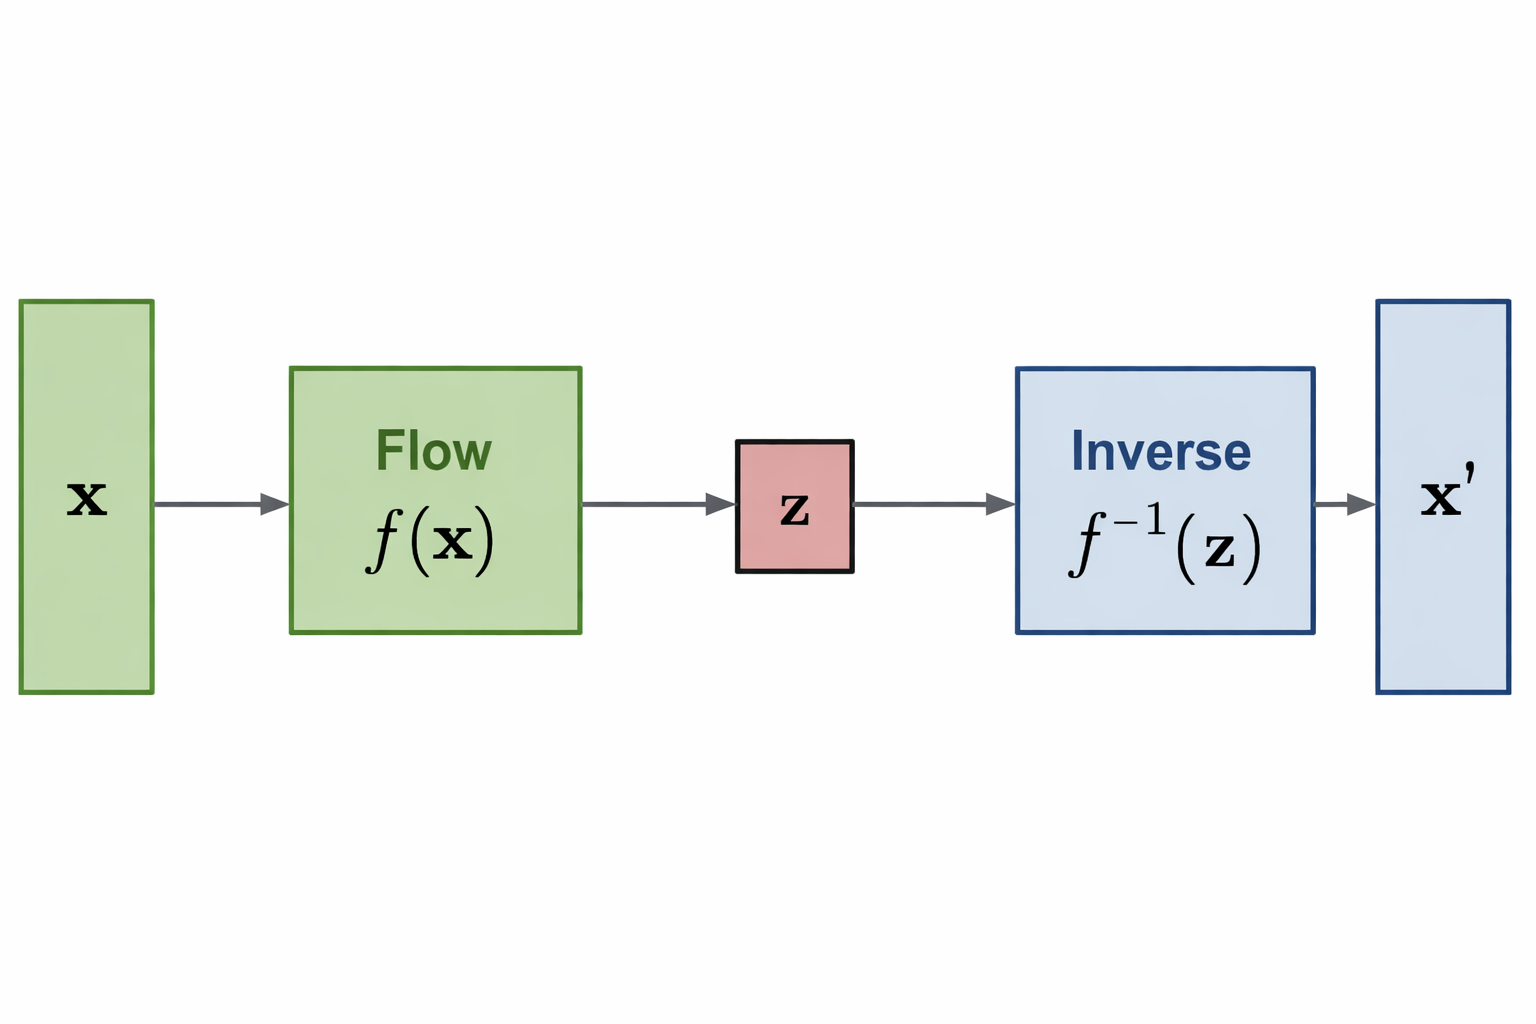
\includegraphics[width=0.6\textwidth]{images/flow.png}
    \caption{Kiến trúc Flow based}
    \label{fig:flowbased}

\end{figure}
Cụ thể, một ảnh chất lượng cao \(x\) được ánh xạ qua chuỗi biến đổi:
\begin{equation}
z = f_K \circ f_{K-1} \circ \cdots \circ f_1(x),
\end{equation}
trong đó \(f_k(\cdot)\) là phép biến đổi khả nghịch tại lớp thứ \(k\) của mô hình Flow, và \(h_{k-1}\) là biến trung gian đầu vào của lớp \(k\), được định nghĩa bởi \(h_0 = x\) và \(h_k = f_k(h_{k-1})\). Sau \(K\) lớp biến đổi, ta thu được biến tiềm ẩn \(z = h_K\), được giả định tuân theo phân phối Gaussian chuẩn \(p(z)\).

Nhờ công thức biến đổi mật độ, hàm likelihood của ảnh \(x\) được tính chính xác như sau:
\begin{equation}
\log p(x) = \log p(z) + \sum_{k=1}^{K}
\log \left|
\det \left(
\frac{\partial f_k(h_{k-1})}{\partial h_{k-1}}
\right)
\right|.
\end{equation}
Trong đó, \(\log p(z)\) đo lường mức độ phù hợp của biểu diễn tiềm ẩn \(z\) đối với phân phối chuẩn, còn các log-định thức Jacobian mô tả sự thay đổi thể tích không gian xác suất qua từng lớp biến đổi. Nhờ thiết kế các phép biến đổi có Jacobian tính toán hiệu quả, mô hình có thể được huấn luyện trực tiếp bằng phương pháp tối đa hóa likelihood.

Trong bài toán khôi phục ảnh, ảnh quan sát \(y\) (bị nhiễu, mờ hoặc giảm độ phân giải) được xem là kết quả của một phép suy biến từ ảnh gốc \(x\). Khi mở rộng sang dạng có điều kiện, các phép biến đổi \(f_k\) được tham số hóa phụ thuộc vào \(y\), cho phép mô hình học phân phối hậu nghiệm \(p(x \mid y)\). Khi đó, quá trình khôi phục ảnh có thể được diễn giải như việc tìm hoặc lấy mẫu các nghiệm \(x\) có likelihood cao.

Đối với các bài toán như denoising, deblurring và đặc biệt là super-resolution, Flow-based models có khả năng sinh ra nhiều ảnh khôi phục khác nhau nhưng đều phù hợp về mặt xác suất với cùng một ảnh quan sát. Nhờ vậy, mô hình không chỉ cải thiện chất lượng khôi phục mà còn mô hình hóa được độ bất định nội tại của bài toán.


